\section{Conversion Stage Data Events} \label{app:data-events}

\captionsetup[table]{list=no}
\captionsetup[figure]{list=no}

\begin{table}[h!]
\centering
\begin{tabular}{r!{\vrule width 1pt}l}
\makecell[r]{\textbf{Description}} & \makecell[l]{\textbf{One or multiple \acs{xml} file(s) are not named based on unified} \\ \textbf{naming format}} \\ \ChangeRT{1pt}
	
\makecell[r]{\textbf{Category}}    & Data Format                         \\ \ChangeRT{0.5pt}
\makecell[r]{\textbf{Severity}}    & \texttt{WARNING}                               \\ \hline
\makecell[r]{\textbf{Handling}}    & \makecell[l]{
	1. Increase \texttt{WARNING} degree counter accordingly \\
	2. Calculate threshold difference, terminate if exceeded \\
	3. Flag file (\texttt{name-warn}) \\
	4. Log warning including file information \\
	5. Continue analytical process \\
}           
\end{tabular}
	\caption{Incorrect Input File Naming}
\end{table}

\begin{table}[h!]
\centering
\begin{tabular}{r!{\vrule width 1pt}l}
\makecell[r]{\textbf{Description}} & \makecell[l]{\textbf{One or multiple \acs{xml} file(s) do not have the} \\ \textbf{appropriate file extension \texttt{.xml}}} \\ \ChangeRT{1pt}
	
\makecell[r]{\textbf{Category}}    & Data Format                         \\ \ChangeRT{0.5pt}
\makecell[r]{\textbf{Severity}}    & \texttt{WARNING}                               \\ \hline
\makecell[r]{\textbf{Handling}}    & \makecell[l]{
	1. Increase \texttt{WARNING} degree counter accordingly \\
	2. Calculate threshold difference, terminate if exceeded \\
	3. Flag file (\texttt{ext-warn}) \\
	4. Log warning including file information \\
	5. Continue analytical process \\
}           
\end{tabular}
	\caption{Incorrect Input File Extension}
\end{table}

\begin{table}[h!]
\centering
\begin{tabular}{r!{\vrule width 1pt}l}
\makecell[r]{\textbf{Description}} & \makecell[l]{\textbf{One or multiple \acs{xml} file(s) are empty}} \\ \ChangeRT{1pt}
	
\makecell[r]{\textbf{Category}}    & Data Format                         \\ \ChangeRT{0.5pt}
\makecell[r]{\textbf{Severity}}    & \texttt{ERROR}                               \\ \hline
\makecell[r]{\textbf{Handling}}    & \makecell[l]{
	1. Remove empty file from analysis \\
	2. Increase \texttt{ERROR} degree counter accordingly \\
	3. Calculate threshold difference, terminate if exceeded \\
	4. Flag file (\texttt{empty-err}) \\
	5. Log error including file information \\
	6. Continue analytical process \\
}           
\end{tabular}
	\caption{Empty Input File}
\end{table}

\begin{table}[h!]
\centering
\begin{tabular}{r!{\vrule width 1pt}l}
\makecell[r]{\textbf{Description}} & \makecell[l]{\textbf{One or multiple \acs{xml} file(s) not of \ac{pos}Log format}} \\ \ChangeRT{1pt}
	
\makecell[r]{\textbf{Category}}    & Data Format                         \\ \ChangeRT{0.5pt}
\makecell[r]{\textbf{Severity}}    & \texttt{ERROR}                               \\ \hline
\makecell[r]{\textbf{Handling}}    & \makecell[l]{
	1. Remove incompatible file from analysis \\
	2. Increase \texttt{ERROR} degree counter accordingly \\
	3. Calculate threshold difference, terminate if exceeded \\
	4. Flag file (\texttt{noPoslog-err}) \\
	5. Log error including file information \\
	6. Continue analytical process \\
}           
\end{tabular}
	\caption{Incompatible (i.e., Non-\ac{pos}Log) File}
\end{table}

\begin{table}[h!]
\centering
\begin{tabular}{r!{\vrule width 1pt}l}
\makecell[r]{\textbf{Description}} & \makecell[l]{\textbf{One or multiple \acs{xml} file(s) are missing required} \\ \textbf{global attribute(s)}} \\ \ChangeRT{1pt}
	
\makecell[r]{\textbf{Category}}    & Data Schema                         \\ \ChangeRT{0.5pt}
\makecell[r]{\textbf{Severity}}    & \texttt{ERROR}                               \\ \hline
\makecell[r]{\textbf{Handling}}    & \makecell[l]{
	1. Remove incorrect file from analysis \\
	2. Increase \texttt{ERROR} degree counter accordingly \\
	3. Calculate threshold difference, terminate if exceeded \\
	4. Flag file (\texttt{glbAttr-err}) \\
	5. Log error including file information \\
	6. Continue analytical process \\
}           
\end{tabular}
	\caption{Input File Missing Required Global Attribute(s)}
\end{table}

\begin{table}[h!]
\centering
\begin{tabular}{r!{\vrule width 1pt}l}
\makecell[r]{\textbf{Description}} & \makecell[l]{\textbf{One or multiple \ac{xml} file(s) have insufficient number} \\ \textbf{of item purchases}} \\ \ChangeRT{1pt}
	
\makecell[r]{\textbf{Category}}    & Data Schema                         \\ \ChangeRT{0.5pt}
\makecell[r]{\textbf{Severity}}    & \texttt{ERROR}                               \\ \hline
\makecell[r]{\textbf{Handling}}    & \makecell[l]{
	1. Remove incorrect file from analysis \\
	2. Increase \texttt{ERROR} degree counter accordingly \\
	3. Calculate threshold difference, terminate if exceeded \\
	4. Flag file (\texttt{item-err}) \\
	5. Log error including file information \\
	6. Continue analytical process \\
}           
\end{tabular}
	\caption{Insufficient Item Purchases in Input File}
\end{table}

\begin{table}[h!]
\centering
\begin{tabular}{r!{\vrule width 1pt}l}
\makecell[r]{\textbf{Description}} & \makecell[l]{\textbf{One or multiple \acs{xml} file(s) are missing required} \\ \textbf{item purchase attribute(s)}} \\ \ChangeRT{1pt}
	
\makecell[r]{\textbf{Category}}    & Data Schema                         \\ \ChangeRT{0.5pt}
\makecell[r]{\textbf{Severity}}    & \texttt{ERROR}                               \\ \hline
\makecell[r]{\textbf{Handling}}    & \makecell[l]{
	1. Remove incorrect file from analysis \\
	2. Increase \texttt{ERROR} degree counter accordingly \\
	3. Calculate threshold difference, terminate if exceeded \\
	4. Flag file (\texttt{itemAttr-err}) \\
	5. Log error including file information \\
	6. Continue analytical process \\
}           
\end{tabular}
	\caption{Input File Missing Required Item Purchase Attribute(s)}
\end{table}

\begin{table}[h!]
\centering
\begin{tabular}{r!{\vrule width 1pt}l}
\makecell[r]{\textbf{Description}} & \makecell[l]{\textbf{One or multiple \acs{xml} file(s) are missing optional} \\ \textbf{item purchase attribute(s)}} \\ \ChangeRT{1pt}
	
\makecell[r]{\textbf{Category}}    & Data Schema                         \\ \ChangeRT{0.5pt}
\makecell[r]{\textbf{Severity}}    & \texttt{WARNING}                               \\ \hline
\makecell[r]{\textbf{Handling}}    & \makecell[l]{
	1. Increase \texttt{WARNING} degree counter accordingly \\
	2. Calculate threshold difference, terminate if exceeded \\
	3. Flag file (\texttt{itemAttr-warn}) \\
	4. Log warning including file information \\
	5. Continue analytical process \\
}           
\end{tabular}
	\caption{Input File Missing Optional Item Purchase Attribute(s)}
\end{table}

\begin{table}[h!]
\centering
\begin{tabular}{r!{\vrule width 1pt}l}
\makecell[r]{\textbf{Description}} & \makecell[l]{\textbf{One or multiple \acs{xml} file(s) are missing required} \\ \textbf{sale information attribute(s)}} \\ \ChangeRT{1pt}
	
\makecell[r]{\textbf{Category}}    & Data Schema                         \\ \ChangeRT{0.5pt}
\makecell[r]{\textbf{Severity}}    & \texttt{ERROR}                               \\ \hline
\makecell[r]{\textbf{Handling}}    & \makecell[l]{
	1. Remove incorrect file from analysis \\
	2. Increase \texttt{ERROR} degree counter accordingly \\
	3. Calculate threshold difference, terminate if exceeded \\
	4. Flag file (\texttt{saleAttr-err}) \\
	5. Log error including file information \\
	6. Continue analytical process \\
}           
\end{tabular}
	\caption{Input File Missing Required Sale Information Attribute(s)}
\end{table}

\begin{table}[h!]
\centering
\begin{tabular}{r!{\vrule width 1pt}l}
\makecell[r]{\textbf{Description}} & \makecell[l]{\textbf{One or multiple \acs{xml} file(s) are missing optional} \\ \textbf{sale information attribute(s)}} \\ \ChangeRT{1pt}
	
\makecell[r]{\textbf{Category}}    & Data Schema                         \\ \ChangeRT{0.5pt}
\makecell[r]{\textbf{Severity}}    & \texttt{WARNING}                               \\ \hline
\makecell[r]{\textbf{Handling}}    & \makecell[l]{
	1. Increase \texttt{WARNING} degree counter accordingly \\
	2. Calculate threshold difference, terminate if exceeded \\
	3. Flag file (\texttt{saleAttr-warn}) \\
	4. Log warning including file information \\
	5. Continue analytical process \\
}           
\end{tabular}
	\caption{Input File Missing Optional Sale Information Attribute(s)}
\end{table}

\begin{table}[h!]
\centering
\begin{tabular}{r!{\vrule width 1pt}l}
\makecell[r]{\textbf{Description}} & \makecell[l]{\textbf{Date in file name does not correspond with \acs{xml} date attribute} \\ \textbf{sale information attribute(s)}} \\ \ChangeRT{1pt}
	
\makecell[r]{\textbf{Category}}    & Data Schema                         \\ \ChangeRT{0.5pt}
\makecell[r]{\textbf{Severity}}    & \texttt{CRITICAL}                               \\ \hline
\makecell[r]{\textbf{Handling}}    & \makecell[l]{
	1. Log error including data information \\
	2. Prompt error information \\
	3. Terminate analytical process
}           
\end{tabular}
	\caption{Input File Name Date Not Corresponding With \acs{xml} Date Attribute}
\end{table}

\begin{table}[h!]
\centering
\begin{tabular}{r!{\vrule width 1pt}l}
\makecell[r]{\textbf{Description}} & \makecell[l]{\textbf{Formatted Python Dictionary is missing} \\ \textbf{file-equivalent attribute(s)}} \\ \ChangeRT{1pt}
	
\makecell[r]{\textbf{Category}}    & Data Schema                         \\ \ChangeRT{0.5pt}
\makecell[r]{\textbf{Severity}}    & \texttt{CRITICAL}                               \\ \hline
\makecell[r]{\textbf{Handling}}    & \makecell[l]{
	1. Log error including data information \\
	2. Prompt error information \\
	3. Terminate analytical process
}           
\end{tabular}
	\caption{Formatted Python Dictionary Missing Attribute(s)}
\end{table}

\begin{table}[h!]
\centering
\begin{tabular}{r!{\vrule width 1pt}l}
\makecell[r]{\textbf{Description}} & \makecell[l]{\textbf{Formatted Python Dictionary value(s) do not comply} \\ \textbf{with file-equivalent value(s)}} \\ \ChangeRT{1pt}
	
\makecell[r]{\textbf{Category}}    & Data Value                         \\ \ChangeRT{0.5pt}
\makecell[r]{\textbf{Severity}}    & \texttt{CRITICAL}                               \\ \hline
\makecell[r]{\textbf{Handling}}    & \makecell[l]{
	1. Log error including data information \\
	2. Prompt error information \\
	3. Terminate analytical process
}           
\end{tabular}
	\caption{Formatted Python Dictionary Value(s) Not Complying with File-Equivalent Value(s)}
\end{table}

\begin{table}[h!]
\centering
\begin{tabular}{r!{\vrule width 1pt}l}
\makecell[r]{\textbf{Description}} & \makecell[l]{\textbf{One or multiple \ac{json} file(s) are corrupted}} \\ \ChangeRT{1pt}
	
\makecell[r]{\textbf{Category}}    & Data Format                         \\ \ChangeRT{0.5pt}
\makecell[r]{\textbf{Severity}}    & \texttt{CRITICAL}                               \\ \hline
\makecell[r]{\textbf{Handling}}    & \makecell[l]{
	1. Log error including file information \\
	2. Prompt error information \\
	3. Terminate analytical process
}           
\end{tabular}
	\caption{\ac{json} Output File(s) Corrupted}
\end{table}

\begin{table}[h!]
\centering
\begin{tabular}{r!{\vrule width 1pt}l}
\makecell[r]{\textbf{Description}} & \makecell[l]{\textbf{One or multiple \ac{json} file(s) are empty}} \\ \ChangeRT{1pt}
	
\makecell[r]{\textbf{Category}}    & Data Format                         \\ \ChangeRT{0.5pt}
\makecell[r]{\textbf{Severity}}    & \texttt{CRITICAL}                               \\ \hline
\makecell[r]{\textbf{Handling}}    & \makecell[l]{
	1. Log error including file information \\
	2. Prompt error information \\
	3. Terminate analytical process
}           
\end{tabular}
	\caption{\ac{json} Output File(s) Empty}
\end{table}

\begin{table}[h!]
\centering
\begin{tabular}{r!{\vrule width 1pt}l}
\makecell[r]{\textbf{Description}} & \makecell[l]{\textbf{One or multiple \ac{json} file(s) are missing} \\ \textbf{file-equivalent attribute(s)}} \\ \ChangeRT{1pt}
	
\makecell[r]{\textbf{Category}}    & Data Format                         \\ \ChangeRT{0.5pt}
\makecell[r]{\textbf{Severity}}    & \texttt{CRITICAL}                               \\ \hline
\makecell[r]{\textbf{Handling}}    & \makecell[l]{
	1. Log error including file information \\
	2. Prompt error information \\
	3. Terminate analytical process
}           
\end{tabular}
	\caption{\ac{json} Output File(s) Missing File-Equivalent Attribute(s)}
\end{table}

\begin{sidewaysfigure}[h!]
	\centering
	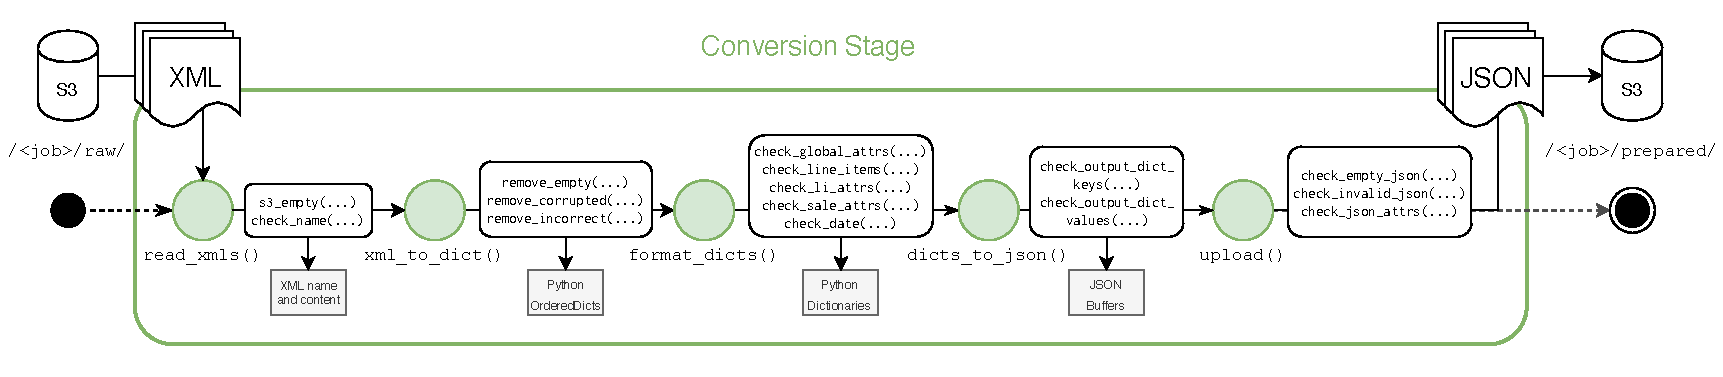
\includegraphics[width=\linewidth]{main-matter/img/5-new-convert}
	\caption{Conversion Stage Overview with Data Handling}
	\label{app:new-convert}
\end{sidewaysfigure}